\documentclass{article}
\usepackage{graphicx} % Required for inserting images
\usepackage[margin=1.0in]{geometry}
\usepackage{float}
\usepackage{hyperref}
\usepackage{listings}

\linespread{1}
\setlength{\parindent}{0pt} % Disable paragraph indentation

\title{CPEN 333: Final Project Report}
\author{Group G6 : Muntakim Rahman and Tomaz Zlindra}
\date{December 6th, 2024}

\begin{document}

\maketitle

\section{Part I : Multithreaded Game}

\subsection{Requirements and Constraints}

We were provided the template with skeleton code (i.e. classes, methods with docstrings) for the implementation of the Snake Game.
The key design structure entailed the following requirement: \\

\textbf{Use Python's \textit{queue} module to ensure multi-producer, multi-consumer achieves synchronization between threads} (i.e. add \textit{dict} items to the queue for "game\_over", "score", "prey", "move"). \\

To program a responsive and thread-safe Snake Game, we use the template data fields and methods for the shown interactions.

\begin{figure}[H]
    \centering
     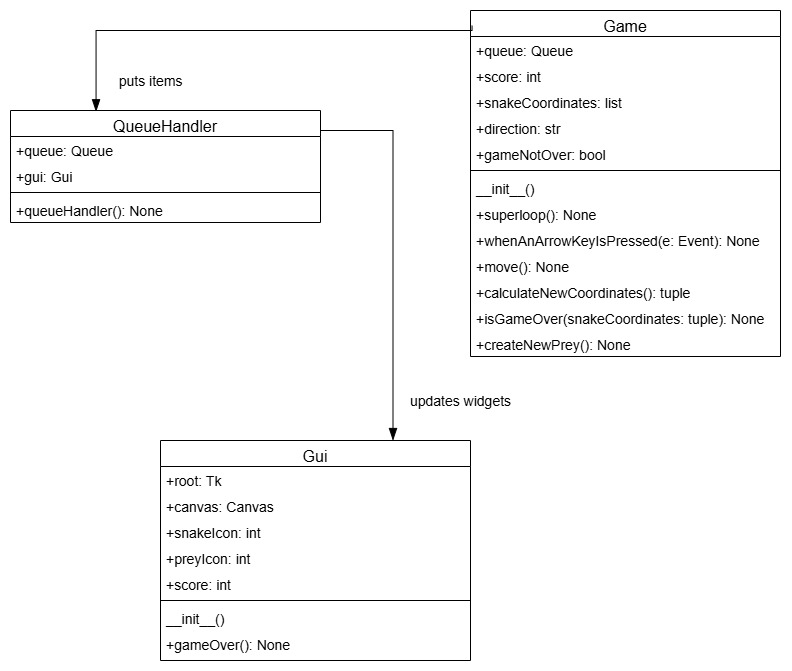
\includegraphics[width=0.8\textwidth]{Part_1_ClassDiagram.jpg}
     \caption{Part 1 : Interactions Between QueueHandler, Game, Gui}
     \label{fig:PreyCapture}
 \end{figure}

\subsection{Structure}


The general structure for Part I was already provided.


We only needed to complete the methods for the "Game" class, such as the superloop, move, calculateNewCoordinates, isGameOver and is createNewPrey methods.

\subsection{Implementation}

\subsubsection{New Snake Coordinates}
This method is very straightforward. It checks the direction by accessing \texttt{self.direction} to determine which direction the head of the snake should travel, and adding/subtracting the \texttt{SNAKE\_ICON\_WIDTH} by the current x or y coordinate.

\subsubsection{Prey Generation}
To generate the prey, we used the \texttt{random} library to generate a random integer for the x direction and the y direction on the Tkinter canvas. We added a small margin so the prey did not generate on or outside the edges of the window.
\subsubsection{Prey Capture}
One of the primary challenges we faced was implementing the prey capture logic. Since prey can spawn at any location on the Tkinter canvas, iterating through a list of tuples to compare coordinates is both resource-intensive and time-consuming. To optimize this process and eliminate the need for nested "for" loops, we calculated the corner coordinates of both the prey and the snake's head. We then checked whether any point of the snake's head fell within the prey's boundaries, as illustrated in figure \ref{fig:PreyCapture}. This method works effectively when the prey is larger than the snake. In cases where the snake is significantly larger than the prey, we reversed the logic: if any point of the prey fell within the snake's boundaries, it would be counted as a collision.
\begin{figure}[H]
   \centering
    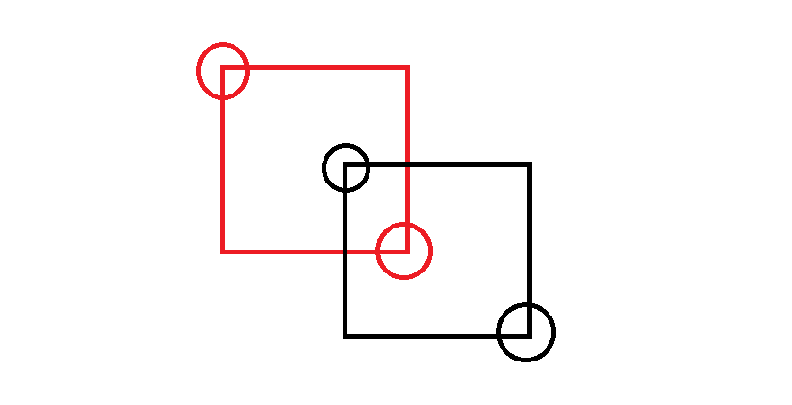
\includegraphics[width=0.6\textwidth]{PreyCapture.png}
    \caption{Prey Capture Criteria : Edge Coordinate Of Prey/Snake Must Be Contained}
    \label{fig:PreyCapture}
\end{figure}

This solution mitigates the amount of recursion performed, while still detecting snake and prey collision.
\subsubsection{Move}
This method completes most the important game logic once the snake moves. Firstly, we had to check whether the prey is captured. If true, we added one to the score, increased the length of the snake, and created a new prey. Otherwise, the length of the snake would not change. Checking if the game is over is also necessary. Tasks are added to the queue are added here so the QueueHandler could manage edits to the GUI.
\subsubsection{Game Over Logic}
The game ends once:
\begin{itemize}
    \item the snake's head either goes out of bounds, OR
    \item the snake runs into itself.
\end{itemize}
We checked whether the coordinates of the snake's head are outside the bounds of the Tkinter canvas or if the head coordinate is the same as any of the other snake coordinates.


\section{Part I Alternative}

\subsection{Modified Approach}
For the Part I Alternative, our one main modification to Part I was to remove the use of the QueueHandler class. This was replaced by the GUI class scheduling GUI updates every 100ms using \texttt{self.root.after(100, self.update)}. Since the GUI and move thread are performing operations simultaneously, we had to add locks to ensure data was not being modified as the changes were being updated by the GUI. The GUI processes used non-blocking locks so none of the GUI methods stalled while waiting for the move thread to either read or write the data.

\end{document}
